\documentclass[]{report}
\usepackage{graphicx}
\usepackage{svg}


% Title Page



\begin{document}
\section*{MapReduce: Simplified Data Processing on Large Clusters}
	This paper by Google is the first paper that introduced MapReduce computation framework.
	
	\subsection*{Programming Model}
		There are two main functions in this framework indicated by the paper: \textit{Map} and \textit{Reduce}. To better understand it, we add another function \textit{Shuffle} into this model, which is widely seen in other description about MapReduce.
		What a \textit{Map} function does is to take an input pair, and process on it to generate a set of intermediate <key, value> pairs.
		The \textit{Shuffle} function groups the generated <key, value> pairs altogether by the same key, and passes them to the \textit{Reduce} function.
		Then for the \textit{Reduce} function, it receives an intermediate key \textit{I} and a set of values for that key. Then it merges these values to form s smaller set of values, typically zero or one values.
		The \textit{Map} and \textit{Reduce} functions are defined by users, so it is actually highly customizable, as long as it still follows the basic paradigm.
	
	
	\subsection*{Implementation}		
		\subsubsection*{Overview}
			\begin{figure}[h]
				\centering
				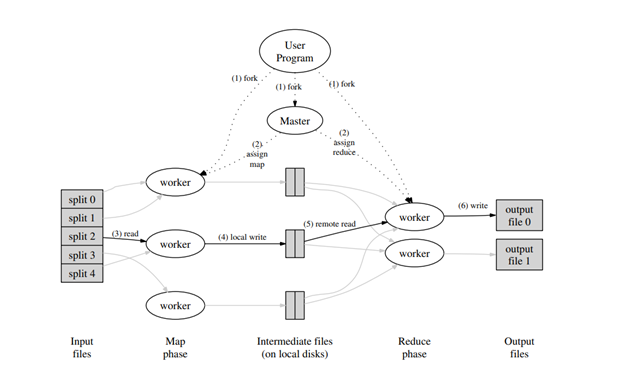
\includegraphics[scale=0.8]{MapReduce.png}
			\end{figure}
		\subsubsection*{Structure}
			The whole model is a \textit{Master-Worker} structured one, meaning that there is a master server that is responsible for working scheduling, and is able to access the global working progress. This master keeps several data strucutres, including the states (idle, in-progress or completed) and identity (Mapper or Reducer) of machines. There is no server that is fixed to be a Map worker or Reduce worker, the workers can be assigned to different tasks dynamically, so that the workloads can be distributed evenly.
		
		\subsubsection{Fault-Tolerance}
			Since MapReduce is used in the context of distributed computation, it has to deal with fault-tolerance issues. In MapReduce, the faults can be from both masters and workers. 
			
			For the workers, the master will ping each worker periodically, and if no response is received from a worker in a certain amount of time, the worker will be marked \textit{failed}. Then a map tasks completed by this failed worker will be reset to \textit{idle} state so that they can be assigned to other workers. And it is similar for a reduce worker. When a worker fails, its map task will be executed by another worker, at the same time, all reduce worker will be notified of this execution, so that they will read from the new worker instead of the previous failed one.
			
			The master will write periodic checkpoints of the master data strucutres, and if the master task dies, a new copy will be started from the latest checkpoint. But when there is only one master, if the master fails, the computation just ends.
			
			With these fault-tolerance mechanism, MapReduce is resilient to large-scale failures.
		
		\subsubsection{Refinement}
			The paper lists several issues that can be improved. For example, imagine that one worker takes a long time to finish the last few tasks of a cluster, then the whole progress will be prolonged, in which the worker becomes a "straggler". In this case MapReduce model can assign the final task to different idle workers, and when one of them finishes, the whole computation ends. This machanism is called \textit{Backup}.
	
	\subsection*{Performance}
		The paper shows the performance of MapReduce on two tasks, one is to search for certain patterns from a large scale of data (1 TB data in experiment), and another is to sort in large scale (1 TB in experiment). The two tasks are representative of most MapReduce programs, which are shuffling data from one representation to another, and information extraction on large scale data. The experiments were run on 1746 machines. For the pattern-searching problem, it showed that only approximately 150 seconds were taken, with about 1 minute of startup overhead. That is to say, beside of the time setting the whole cluster to work, it took a relatively short time to process the data on a large amount of machines distributedly. For the sort task, the entire computation took 891 seconds. However, with the Backup machanism disabled, the running time will excceed to 1283 seconds, with an increase of 44\%. This was caused by the "straggler" workers mentioned above. And when 200 processes are killed manually, the whole computation only took 5\%more of the normal time, which showed that MapReduce model is robust against machine failures.
	
	\subsection*{Experience}
		When MapReduce library was released, instances that utilizes this computation model increases dramatically in Google, including large-scale machine learning problems, data extraction, etc. It became popular because this model enables programmers with limited experience in distributed or parallel computing to have access to large scale of computation resources, and takes only a short time to write a simple code that can be efficiently run on large amount of machines. This greatly accelerated developments. This is guranteed by the implementation of MapReduce library, because the library itself has already optimized data passing, and dealt automatically with the most difficult part of coding against failures.
	
	
	\subsection*{Comment}
		This paper is mainly focused on the MapReduce model, which puts a majority of its attention on \textit{Map} andd \textit{Reduce}. However, in practice, the MapReduce model is built on a distributed file system (DFS), which lays the foundation for \textit{Shuffle} process.
		
		MapReduce is a simple model, it tries to split complicated computation tasks into basic ones in the form of \textit{Map} and \textit{Reduce}, to lower the complexity of implementation. In fact, the complexity is transfered to the implementation of MapReduce library.
		
		However, MapReduce programs resemble batch processing programs, that it needs a relatively complete input to start. Each computation requires at least 2 disk I/Os. This causes a long waiting time for each computation, and cannot achieve the objective that responds quickly in industry.
		
		After all, even though MapReduce seems a somehow outdated nowadays, by the time it is proposed, it was a efficient computation model considering Google's industry requirement at that time.


\newpage
\section*{A Model of Computation for MapReduce}
	After MapReduce was proposed by Google since 2004, it was widely used in many companies. This paper intends to take a deeper analysis into MapReduce, which is to propose a model of parallel computation using MapReduce paradigm, and tries to prove its ability to simulate PRAM algorithms.
	
	\subsection*{MapReduce Programming Paradigm}
		The paper defines a MapReduce Programming Pradigm, it gives a formal definition on mappers and reducers first. It is emphasized that a mapper operates on one <key, value> pair at a time, and that mappers can manipulate keys arbitrarily while reducers cannot change the keys at all. Then the paper describes the process that the system executes MapReduce computations: the Map functions are executed first, and then shuffle the <key, value> pairs to reducers, and reduce functions are executed after then. When the last reducer halts, the whole computation ends. 
		
	\subsection*{MapReduce Class (MRC)}
		To better define the MapReduce Class, the paper assumes that the input to any mapper or reducer is substantially sublinear in the size of the data. In other words, the memory of single machine cannot support process of a large amount of data, otherwise the computation can be solved with single mapper and reducer. Similarly, the number of machines is restricted. Moreover, the number of Map Reduce rounds is limited, because shuffling is time-comsuming. The MRC is defined as follows: given a finite sequence of pairs <$k_{j}, v_{j}$> as input, the length of the input is $n=\sum_{j}(|k_{j}|+|v_{j}|)$. Fixing an $\epsilon>0$, an algorithm in $MRC^{i}$ consists of a sequence $\left\langle\mu_{1}, \rho_{1}, \mu_{2}, \rho_{2}, \ldots, \mu_{R}, \rho_{R}\right\rangle$ of operations which outputs the correct answer with probablity at least $\frac{3}{4}$ where: each $\mu_{r}$ is a randomized mapper with O($\log n$)-length words that uses O($n^{1-\epsilon}$) space and time polynomial in $n$, each $\rho_{r}$ is a randomized reducer with O($\log n$)-length words that uses O($n^{1-\epsilon}$) space and time polynomial in $n$. The total space used by the pairs output by $\mu_{r}$ is O($n^{2-2\epsilon}$), and the number of rounds $R=O(\log^{i}n)$. A DMRC is a deterministic variant of MRC, since randomization in MRC is allowed. A mapper runs one pair at a time is emphasized again, and remembers nothing about previous pairs. This is mentioned because each reducer may get a sequence of values in arbitrary orders, and the correctness will be ensured by following the restriction.
		
		For the machine restriction, each key gets mapped to a unique reducer instance, and since the total number of distinct keys can be as large as O($n^{2-2\epsilon}$), the total number of reduce instances can be the same. Thus it can be possible that more than one instance of a reducer may be run on the same machine. The restrictions are justified in the paper, so that the definition on MRC can be reasonable.
	\subsection*{Related Work}
		The paper compares MapReduce with PRAM, because PRAM was the most prevalent model in theoretical studying. Although PRAM models are attracting in theory, by the time the paper was published, there was no fully shared-memory machines with large numbers of processors, and the simultation was slow.
		
		It is seemingly that MapReduce is very well suited for simple and naive parallelization, such as words counting. But in fact many complicated MapReduce algorithms deployed on difficult tasks had been proposed. It reflected the power of the MapReduce model, but these works did not define the framework under which they should be analyzed.
	\subsection*{Finding an MST of a Dense Graph Using MapReduce}
		
	\subsection*{Algorithmic Design Technique for MRC}
	
	\subsection*{Simulating PRAMs via MapReduce}
		The paper shows that any \textit{CREW PRAM} algorithm using O($n^{2-2\epsilon}$) total memory and processors, and $t=t(n)$ time can be run in O($t$) rounds in DMRC. The paper uses O($n^{2-2\epsilon}$) reducers where one reducer simulates each processor used in PRAM, and another simulates each memory location used by PRAM algorithm. The mappersa are used to route memory requests and send required memory lines to reducers. Each reducer then does a step of computation for each PRAM processor, and writes into memory, and then requests a new one. The process will repeat.
	
	\subsection*{Comments}
		Thee paper only proves the workability of DMRC, which is only part of MRC.
\end{document}          
